\section{Flatten}
Giriş verilerini tek boyutlu bir vektöre dönüştürür. Convolution ve Pooling katmanlarından gelen matrisleri tek boyutlu diziye çevirir. Böylece veriyi tam bağımlı katmana hazırlar.

\begin{figure}[h]
    \centering
    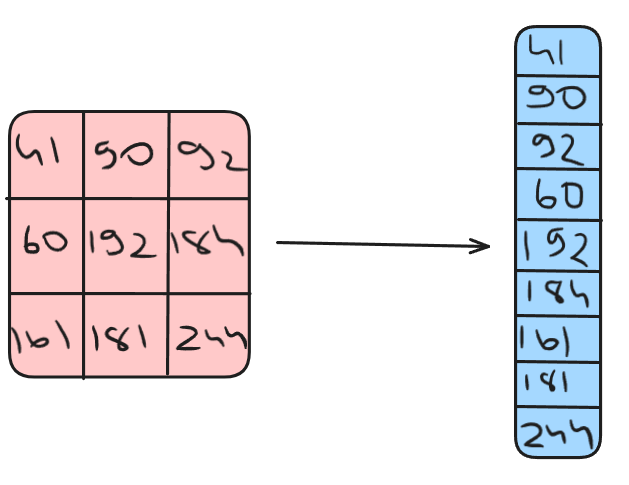
\includegraphics[width=1\textwidth]{images/flatten_layer.png}
    \caption{Flatten katmanı.}
    \label{fig:enter-label}
\end{figure}

\newpage